\chapter{Einleitung}
\pagenumbering{arabic} % ab jetzt die normale arabische Nummerierung

Die synthetische Erzeugung von Höhendaten zur Darstellung von möglichst realistischen Landschaften fand insbesondere nach der Vorstellung einer Rauschfunktion\footnote{Auch bekannt als \emph{Perlin-Noise}} von Ken Perlin 1985\cite{PERLIN1985} viel Aufmerksamkeit. Zwar gab es in den letzten Jahren nur noch wenige Veröffentlichungen zu dem Thema, allerdings kam ein neues Feld auf in dem die prozedurale Erzeugung von natürlichen Strukturen eine große Rolle spielt - die Computerspiele.

Die prozedurale Generierung ihrer Landschaften bietet den Entwicklern viele Vorteile. 
So lassen sich Zeit und Personalkosten sparen, die sonst in Ausgestaltung der Landschaftsdetails fließen würde, was es ermöglicht nahezu unendliche Spielwelten mit einmaligem Aussehen zu erschaffen.
Als bekanntestes Beispiel ist hier sicherlich das Spiel Minecraft vom Studio Mojang zu nennen, welches einen großteil seiner Faszination aus der komplett prozedural erzeugten veränderbaren Landschaft zieht.

Im folgenden werden 3 bewährte Algorithmen zur Erzeugung von Höhenfeldern vorgestellt und daraufhin untersucht, in wie weit sie zur Speicherung einer nahezu unendlich großen Landschaft wie in Minecraft geeignet sind.
Zuerst wird der Diamond-Square Algorithmus\cite{DiamondSquare} vorgestellt, welchen man verallgemeinert auch als einen \emph{Polygon unterteilungs Algorithmus} bezeichnen kann. Danach wird kurz die Spektalsynthese mit der Fourier-Methode erläutert bevor es eine Einführung in die Welt der Rauschfunktionen gibt. 
Neben der Synthese von Landschaften sind diese Algorithmen vielseitig einsetzbar. Insbesondere bei der bereits erwähnten Kategorie der Rauschfunktionen ist davon auszugehen, dass sie auch in proprietärer 3D-Software wie Computerspielen trotz ihres Alters noch als wichtiger Algorithmus genutzt wird. Dies liegt vor allem an ihrer Flexibilität sowie Skalierbarkeit in mehreren Dimensionen durch die auch Wolken, Feuer, Rauchverwirbelung und sogar Fellverteilung dargestellt werden kann\cite{texturingAndModeling}.

Der Diamond-Square Algorithmus sowie verschiedene Rauschfunktionen sind in dem diesem Dokument beiliegendem Unity-Projekt in C\# bzw. HLSL\footnote{High Level Shading Language} implementiert und lassen sich durch Unity auf Windows, Unix und Mac OS basierten Betriebssystemen kompilieren.

%TODO Kapitel zu aktuellen Anwendungen

\section{Datenstrukturen zur Landschaftsspeicherung: Höhenfelder vs. Voxel}
Landschaften werden in der Regel entweder in einem Höhenfeld oder in Voxeln gespeichert.
Der wesentliche Unterschied der beiden Techniken liegt in ihrer Dimensionen. Das Höhenfeld speichert in einem ganzzahligen Zweidimensionalen Koordinatensystem zu jedem Punkt den dazugehörigen Höhenwert der Landschaft, während ein Voxel den Dichtewert eines Punktes in einem Dreidimensionalem Koordinatensystem darstellt. Beide Datenstrukturen haben den Vorteil, dass sich die Position jedes Wertes in der Landschaft implizit aus der Position zu seinen Nachbarn bestimmen lässt. Eine zusätzliche Speicherung seiner Koordinate ist also nicht notwendig. Anders wäre es bei Polygonen, wo jeder Vertex eine Koordinate im Raum hat. Polygone sind daher gut für Szenen geeignet, in denen viel Leerraum herrscht, welcher in den hier vorgestellten Datenstrukturen zu unnötig gespeicherten Daten führe würde

\subsection{Höhenfelder}
Die meisten Algorithmen beziehen sich auf die Erzeugung von Landschaften mit Hilfe von Höhenfeldern. Dies ist vermutlich vor allem dem geschuldet, dass viele Algorithmen recht alt sind und sich Voxel basierte Verfahren aufgrund des Speicherplatzmangels nicht lohnten.
Auch wenn Höhenfelder bereits zu sehr realistischen Ergebnissen großer Landschaftsstriche führen, haben sie einen entscheidenden Nachteil. Da pro Punkt im Koordinatensystem nur ein Höhenwert gespeichert werden kann sind Höhlen oder Überhänge nicht möglich.

Aufgrund der vereinfachten Algorithmen und der großen Verbreitung wird sich im folgendem auf Höhenfelder beschränkt. Eine Erweiterung in die dritte Dimension ist mit dem Ansatz der Rauschfunktionen\ref{Noise} jedoch problemlos möglich.
Ein weiterer Vorteil von Höhenfeldern ist, dass sich durch die simple Verbindung nebeneinanderliegender Punkte sehr einfach ein Polygon erzeugen lässt, welches Hardwarebeschleunigt gerendert werden kann.

\begin{figure}
	\centering
	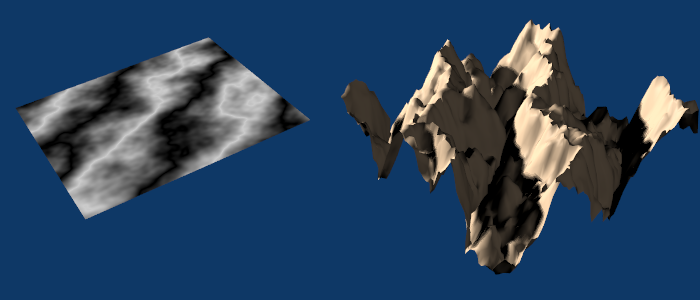
\includegraphics[width=\textwidth]{images/heightfield_rendered.png}
	\caption{Gegenüberstellung einer Heightfield als Textur(links) und der resultierenden Landschaft. Bildquelle: http://tinyurl.com/zu7gond}\label{img.heightfield}
\end{figure}

\subsection{Voxel}
Der Begriff Voxel leitet sich aus den Begriffen Volumen und Pixel ab.
Durch die Speicherung in einem dreidimensionalem Koordinatensystem wird nun auch die, bei den Höhenfeldern explizit gespeicherte, Höhe eines Punktes implizit gespeichert. Dies ermöglicht es eine weitere Information für jeden Punkt explizit zu speichern. In der Regel ist dies ein Dichtewert der es ermöglicht verschiedene Arten von Materialien zu simulieren.

Um Voxel hardwarebeschleunigt zu rendern müssen auch diese in ein Polygon umgewandelt werden. Dies funktioniert normalerweise über Raycasting oder den Marching Cube Algorithmus.

\begin{figure}
	\centering
	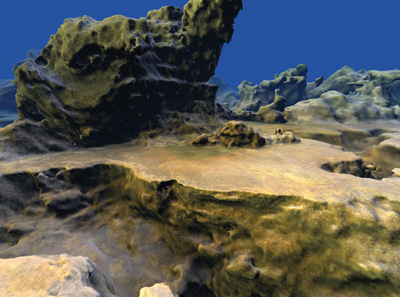
\includegraphics[width=\textwidth]{images/voxel_rendered.jpg}
	\caption{Gerenderte Voxellandschaft mit Überhängen. Bildquelle: http://tinyurl.com/jq8vta8}\label{img.heightfield}
\end{figure}

\section{Implizite vs. explizite Funktionen}
Alle hier vorgestellten Methoden lassen sich in 2 Gruppen einteilen: implizite und explizite Funktionen.
Während eine explizite Funktion alle Höhenpunkte auf einmal berechnet lässt sich die implizite Funktion für jeden Punkt, also jede Koordinate, isoliert auswerten. 

Durch die Unabhängigkeit der Berechnung für jeden einzelnen Punkt lassen sich implizite Algorithmen sehr effizient parralel auf einer GPU berechnen\footnote{Siehe Beispielimplementierung in einem Vertex-Shader}. Dies ermöglicht die Ausführung zur Laufzeit, während explizite Methoden in der Regel vor oder bei Programmstart einmalig berechnet werden und deren Ergebnisse in einer Textur gespeicher werden.
Dies hat den Vorteil, dass der Speicherbedarf teilweise enorm sinken kann. 

Ein Einsatzgebiet für diese Technik ist das Bump-Mapping bzw. Displacement Mapping bei der zusätzliche Höhenwerte auf ein Objekt durch Shading oder neue Vertices auf der Objektoberfläche hinzugefügt werden\cite{displacementNStuff}. Da moderne Echtzeitspiele immer mehr und immer größere Texturen verwenden steigt der Bedarf an Speicher enorm wenn für jede Textur noch eine Normal/Bump/Displacement Map gespeichert werden muss. Implizite Methoden erlauben es, anstatt der Texturen einige Parameter in Form von Floats und Integern zu speichern.
Auch eine Anpassung des Detailgrades ist zur Laufzeit ohne Probleme möglich, während bei der Detailgrad bei expliziten Methoden von der Auflösung der Textur abhängt\footnote{Diese Eigenschaften lassen sich zwar auch durch die Berechnung von expliziten Methoden zur Laufzeit erreichen, jedoch lassen diese sich wie erwähnt nicht effektiv durch die GPU beschleunigen wodurch die Berechnung innerhalb eines Frames unperformant ist.}.

Der Diamond-Square Algorithmus sowie die Spektralsynthese gehören zu der Gruppe der expliziten Algorithmen, während die Rauschfunktionen implizit auswertbar sind.